\documentclass[11pt]{article}

\usepackage[margin=1in]{geometry}
\usepackage{graphicx}
\usepackage{subcaption}
\usepackage{booktabs}
\usepackage{float}
\usepackage{array}
\usepackage{amsmath}
\usepackage{tikz}
\usepackage{hyperref}
\usetikzlibrary{arrows.meta,positioning,shapes.geometric}

\title{ABIDES Daily Investor Baselines and Parameter Sweep Results}
\author{Belief-Aware RL Project}
\date{\today}

\begin{document}
\maketitle

\section{Research Goal and Report Roadmap}

The central question is whether an RL trader can make better decisions by
estimating a latent belief over the market participants it is trading against.
In a real market, the agent does not observe each participant's strategy
directly. It only observes public market data such as prices, spreads, order
book imbalance, volume, and recent returns. The goal is therefore not to
identify every individual trader, but to infer enough about the hidden market
composition to choose better actions.

Formally, we want to learn a belief-conditioned trading policy:
\[
    b_t = P(\text{market regime or participant mix} \mid \text{public history up to } t),
    \qquad
    a_t = \pi(o_t, b_t),
\]
where \(o_t\) is the usual market observation and \(b_t\) is an online estimate
of whether the current market is more noise-dominated, momentum-dominated, or
mean-reversion-dominated. A standard RL agent only sees \(o_t\). A belief-aware
agent sees both \(o_t\) and \(b_t\).

\subsection{What Are We Trying To Do?}

We are trying to test whether public market data contains enough information to
infer useful hidden structure about the agents generating the market. If the
market is dominated by momentum traders, then following short-horizon pressure
may be profitable. If the market is dominated by value or mean-reversion
traders, then fading short-term moves may be better. A fixed policy averages
across these regimes. A belief-aware policy should adapt as its estimate of the
current regime changes.

\subsection{What Experiments Are We Running?}

This report studies two preliminary experiments that set up the belief-aware RL
question.

First, we run a fixed baseline benchmark in the ABIDES daily-investor
environment. Six hand-coded strategies trade in the same AAPL-calibrated market:
\texttt{HOLD}, \texttt{BUY\_HOLD}, \texttt{RANDOM}, \texttt{MOMENTUM},
\texttt{MR}, and \texttt{MR\_INV}. This tells us which simple signals the
default market rewards.

Second, we run one-at-a-time parameter sweeps over the background market and
environment settings. These sweeps change the number and strength of value
agents, momentum agents, noise agents, market-maker settings, order size, and
timestep duration. The purpose is to check whether changing hidden market
composition changes which strategy performs best.

\subsection{How Do These Results Help?}

The baseline and sweep results are not yet the final belief-aware RL experiment.
They are the diagnostic layer that tells us whether belief estimation is worth
doing. If every market composition rewarded the same strategy, then estimating
the hidden participant mix would add little value. But if different
compositions favor different behavior, then a belief module has a real signal
to exploit.

The current results support that motivation. The default AAPL calibration is
strongly momentum-friendly: the \texttt{MOMENTUM} heuristic outperforms the
mean-reversion heuristics by a wide margin. The value-agent sweep then shows
the direction we care about: increasing fundamental anchoring makes
mean-reversion more competitive and weakens momentum. This is exactly the kind
of regime dependence a belief-aware policy should learn to detect from public
history.

\subsection{What Are The Next Steps?}

The next step is to replace hand-coded strategy selection with a learned
belief-conditioned policy. Concretely, we should:

\begin{enumerate}
    \item Define a small set of latent market regimes, such as
    noise-dominated, momentum-dominated, value-agent-dominated, and mixed.
    \item Generate ABIDES training data from each regime while exposing only
    public market observations to the learning agent.
    \item Train a belief module that maps recent public history to a regime
    belief vector.
    \item Train and compare two RL traders: a baseline policy
    \(\pi(o_t)\), and a belief-aware policy \(\pi(o_t, b_t)\).
    \item Evaluate both trading performance and belief quality using P\&L,
    Sharpe ratio, drawdown, win rate, and belief accuracy against the known
    simulated regime.
\end{enumerate}

The rest of this document follows that flow. The setup sections explain the
ABIDES market, the trading interface, and the heuristic policies. The results
sections show which policies work under the default calibration and how those
rankings shift under parameter sweeps. The conclusion translates those findings
into the next belief-aware RL implementation plan.

\textbf{We will then expand this to a multi-agent setting, where the agent is trading against a pool of other agents, each with their own unique strategy.}

\section{Experimental Setup}

The experiment evaluates the \texttt{markets-daily\_investor-v0} ABIDES-Gym
environment under an AAPL-calibrated \texttt{rmsc04} background market. The
daily investor chooses among three actions at each step: market buy, hold, or
market sell. Performance is measured by final mark-to-market P\&L relative to
the starting cash account.

The baseline benchmark uses 50 episodes per strategy with a 60 second timestep,
starting cash of 1,000,000 cents, and fixed order size of 10 shares. All P\&L
numbers below are in cents.

\begin{figure}[H]
\centering
\resizebox{\linewidth}{!}{%
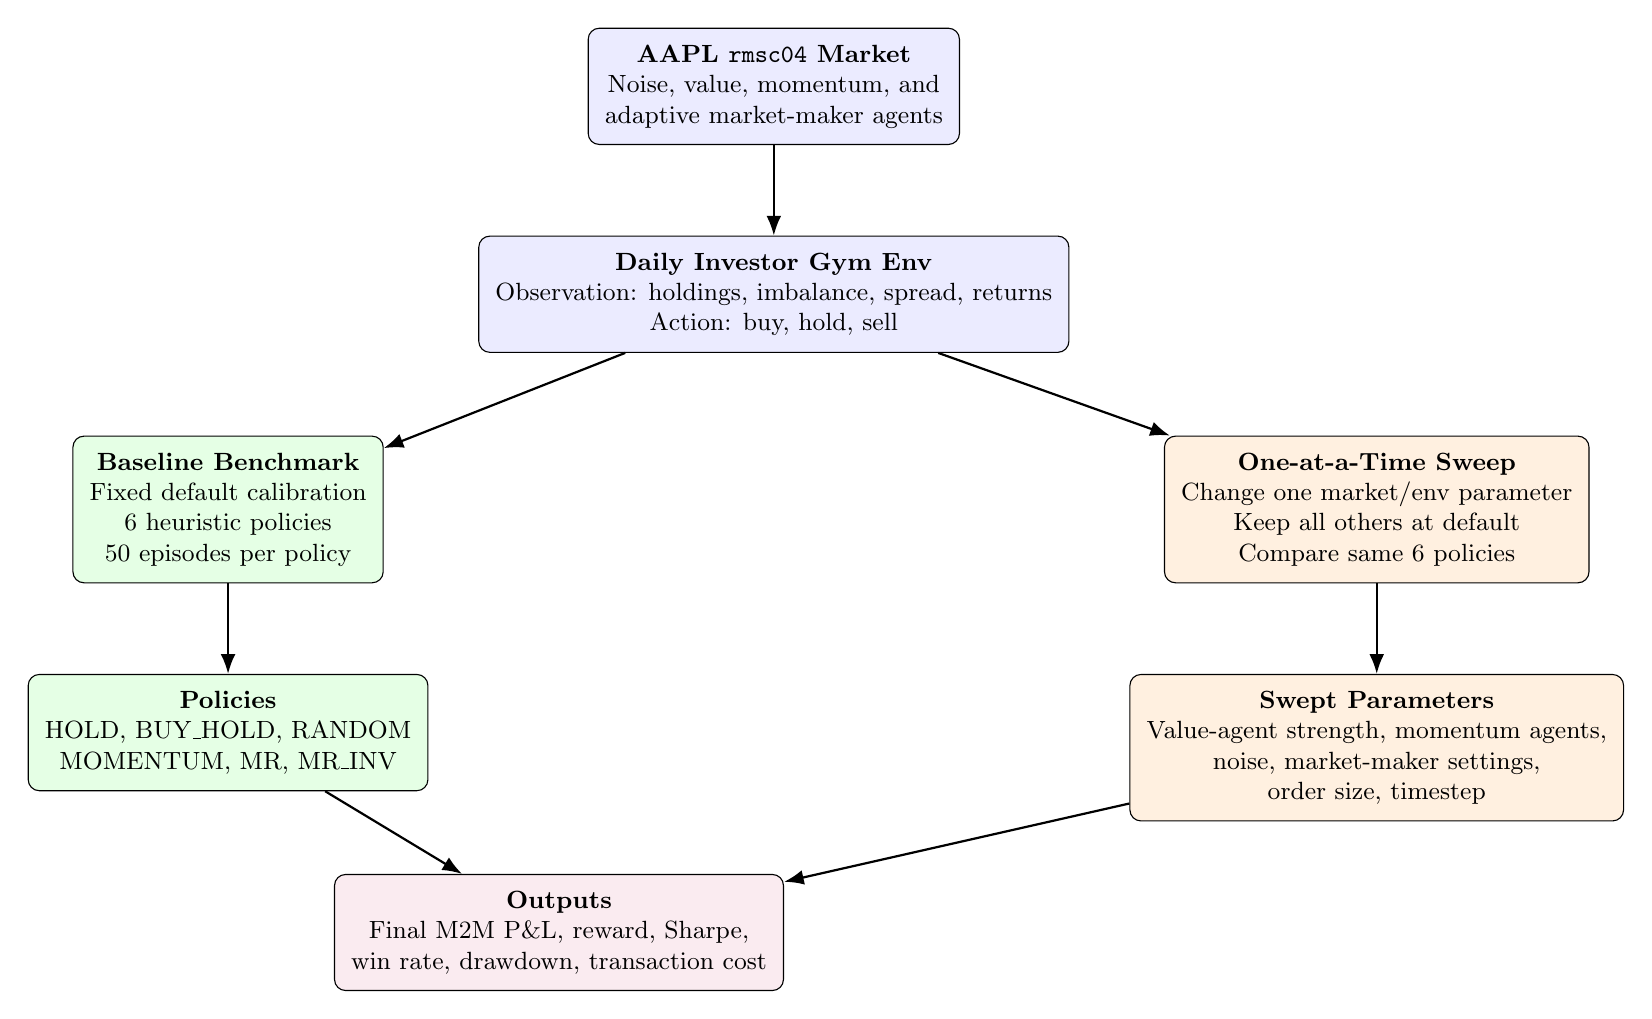
\begin{tikzpicture}[
    font=\small,
    node distance=1.15cm and 1.45cm,
    box/.style={
        draw,
        rounded corners,
        align=center,
        minimum width=3.2cm,
        minimum height=0.95cm,
        inner sep=6pt
    },
    env/.style={
        box,
        fill=blue!8,
        minimum width=4.4cm
    },
    baseline/.style={
        box,
        fill=green!10
    },
    sweep/.style={
        box,
        fill=orange!12
    },
    metric/.style={
        box,
        fill=purple!8,
        minimum width=3.7cm
    },
    arrow/.style={
        -{Latex[length=2.5mm]},
        thick
    }
]

\node[env] (market) {
    \textbf{AAPL \texttt{rmsc04} Market}\\
    Noise, value, momentum, and\\
    adaptive market-maker agents
};

\node[env, below=of market] (gym) {
    \textbf{Daily Investor Gym Env}\\
    Observation: holdings, imbalance, spread, returns\\
    Action: buy, hold, sell
};

\node[baseline, below left=1.05cm and 1.2cm of gym] (baseline) {
    \textbf{Baseline Benchmark}\\
    Fixed default calibration\\
    6 heuristic policies\\
    50 episodes per policy
};

\node[sweep, below right=1.05cm and 1.2cm of gym] (sweep) {
    \textbf{One-at-a-Time Sweep}\\
    Change one market/env parameter\\
    Keep all others at default\\
    Compare same 6 policies
};

\node[baseline, below=of baseline] (policies) {
    \textbf{Policies}\\
    HOLD, BUY\_HOLD, RANDOM\\
    MOMENTUM, MR, MR\_INV
};

\node[sweep, below=of sweep] (params) {
    \textbf{Swept Parameters}\\
    Value-agent strength, momentum agents,\\
    noise, market-maker settings,\\
    order size, timestep
};

\node[metric, below right=1.05cm and -1.2cm of policies] (metrics) {
    \textbf{Outputs}\\
    Final M2M P\&L, reward, Sharpe,\\
    win rate, drawdown, transaction cost
};

\draw[arrow] (market) -- (gym);
\draw[arrow] (gym) -- (baseline);
\draw[arrow] (gym) -- (sweep);
\draw[arrow] (baseline) -- (policies);
\draw[arrow] (sweep) -- (params);
\draw[arrow] (policies) -- (metrics);
\draw[arrow] (params) -- (metrics);

\end{tikzpicture}%
}
\caption{Experimental design. The baseline benchmark evaluates six fixed
heuristics under the default AAPL calibration. The sweep keeps the same policy
set but changes one environment or background-market parameter at a time to
identify which market regimes favor momentum or mean reversion.}
\label{fig:experiment-design}
\end{figure}

\section{Setup Context}

The daily investor is not trading against a simple price process. It trades
inside an agent-based limit-order-book simulation. The background agents create
order flow, liquidity, and price movement; the daily investor observes the
resulting market state and submits one market order decision per environment
step.

\subsection{Background Market Agents}

\begin{table}[H]
\centering
\small
\begin{tabular}{p{0.22\linewidth}p{0.68\linewidth}}
\toprule
Agent type & Role in the simulated market \\
\midrule
Noise agents &
Submit random buy or sell orders. They create uninformed order flow and volume,
which affects book depth, spread costs, and short-horizon price noise. \\
Value agents &
Trade when the market price deviates from their belief about fundamental value.
More active value agents tend to anchor prices and make the market more
mean-reverting. \\
Momentum agents &
Trade with short-horizon trends, typically buying after upward movement and
selling after downward movement. More momentum activity can make price moves
persist instead of immediately reverting. \\
Adaptive market makers &
Continuously provide bid and ask liquidity around the current market. Their
wake-up frequency, spread rule, and sizing determine how costly it is for the
daily investor to cross the spread. \\
\bottomrule
\end{tabular}
\caption{Background agents in the \texttt{rmsc04} market configuration.}
\label{tab:background-agents}
\end{table}

\subsection{Daily Investor Interface}

At each step, the daily investor receives a compact observation vector derived
from the order book and its own portfolio, then chooses one of three actions.

\begin{table}[H]
\centering
\small
\begin{tabular}{llp{0.56\linewidth}}
\toprule
Quantity & Location & Meaning \\
\midrule
Holdings & \texttt{obs[0]} & Current signed share inventory. Positive means long,
negative means short. \\
Imbalance & \texttt{obs[1]} & Bid volume divided by total visible bid and ask volume.
Values above 0.5 indicate stronger bid-side pressure. \\
Spread & \texttt{obs[2]} & Best ask minus best bid, in cents. This is the immediate
cost paid by market orders. \\
Direction feature & \texttt{obs[3]} & Difference between mid price and last
transaction price, a short-horizon microstructure signal. \\
Recent returns & \texttt{obs[4:7]} & Lagged mid-price returns used by the
momentum and mean-reversion heuristics. \\
\bottomrule
\end{tabular}
\caption{Observation features used by the daily investor environment.}
\label{tab:observation-context}
\end{table}

The action space is deliberately simple: \texttt{0} submits a market buy,
\texttt{1} holds, and \texttt{2} submits a market sell. Because these are market
orders, active strategies pay spread and slippage whenever they trade.
\texttt{HOLD} is therefore the zero-trading control: it should have exactly zero
P\&L in this setup.

\subsection{Baseline Policies}

The baseline policies are simple hand-coded trading rules. They are not trained
RL agents; they are reference points that show which types of signals the market
currently rewards.

\begin{table}[H]
\centering
\small
\begin{tabular}{p{0.18\linewidth}p{0.72\linewidth}}
\toprule
Policy & Trading rule and interpretation \\
\midrule
\texttt{HOLD} &
Never trades. This is the sanity-check baseline: final P\&L should remain zero
because cash and holdings never change. \\
\texttt{BUY\_HOLD} &
Buys once at the start and then holds. This measures whether the simulated day
has a directional long bias. \\
\texttt{RANDOM} &
Chooses buy, hold, or sell uniformly at random. This is a noisy lower bound for
active trading because it pays transaction costs without using a signal. \\
\texttt{MOMENTUM} &
Follows order-book pressure. If bid-side imbalance is high, it buys; if ask-side
pressure is high, it sells. The hypothesis is that current order-book pressure
predicts near-future price movement in the same direction. \\
\texttt{MR} &
Mean reversion. It fades recent mid-price returns: after a price drop it buys,
and after a price rise it sells. The hypothesis is that short-horizon moves
overshoot and then revert. \\
\texttt{MR\_INV} &
Mean reversion with an inventory cap. It uses the same signal as \texttt{MR} but
stops adding to positions once inventory gets too large. This tests whether
mean-reversion losses are caused mainly by uncontrolled position buildup. \\
\bottomrule
\end{tabular}
\caption{Hand-coded baseline policies evaluated in both the fixed benchmark and
the parameter sweep.}
\label{tab:baseline-policy-context}
\end{table}

\subsection{How To Interpret the Sweep}

The sweep changes one parameter at a time while keeping all other parameters at
their default AAPL calibration. This isolates directional effects: for example,
increasing \texttt{num\_value\_agents} tests whether stronger fundamental
anchoring makes mean reversion more profitable, while increasing
\texttt{num\_momentum\_agents} tests whether trend-following background flow
makes momentum more profitable. Since the sweep plots show mean P\&L with one
standard deviation error bars, wide overlapping intervals should be interpreted
as high uncertainty rather than a decisive ranking.

\section{Baseline Strategy Results}

\begin{table}[H]
\centering
\small
\begin{tabular}{lrrrrrr}
\toprule
Strategy & Mean P\&L & Std. P\&L & Sharpe & Win Rate & Mean DD & Txn. Cost \\
\midrule
HOLD      &       0.00 &      0.00 &  0.000 & 100.0\% & 0.000 &   0.00 \\
BUY\_HOLD &    -643.20 &   7336.97 & -0.088 &  46.0\% & 0.009 &   1.25 \\
RANDOM    &    6033.86 &  63751.45 &  0.095 &  58.0\% & 0.072 & 351.80 \\
MOMENTUM  &   66171.66 & 131290.71 &  0.504 &  82.0\% & 0.122 & 371.30 \\
MR        &  -57942.00 & 120705.01 & -0.480 &  36.0\% & 0.140 & 462.57 \\
MR\_INV   &  -54810.98 &  26958.35 & -2.033 &   2.0\% & 0.062 & 375.60 \\
\bottomrule
\end{tabular}
\caption{Baseline performance over 50 episodes. Sharpe is computed as mean
final P\&L divided by standard deviation of final P\&L across episodes.}
\label{tab:baseline-results}
\end{table}

The baseline result is clear: the default market regime is momentum-friendly
and not mean-reversion-friendly. \texttt{MOMENTUM} has the highest mean P\&L,
the best Sharpe ratio, and an 82\% win rate. The mean-reversion policies lose
money on average. \texttt{MR\_INV} reduces variance and drawdown relative to
plain \texttt{MR}, but it is still consistently negative, with only a 2\% win
rate.

\begin{figure}[H]
\centering
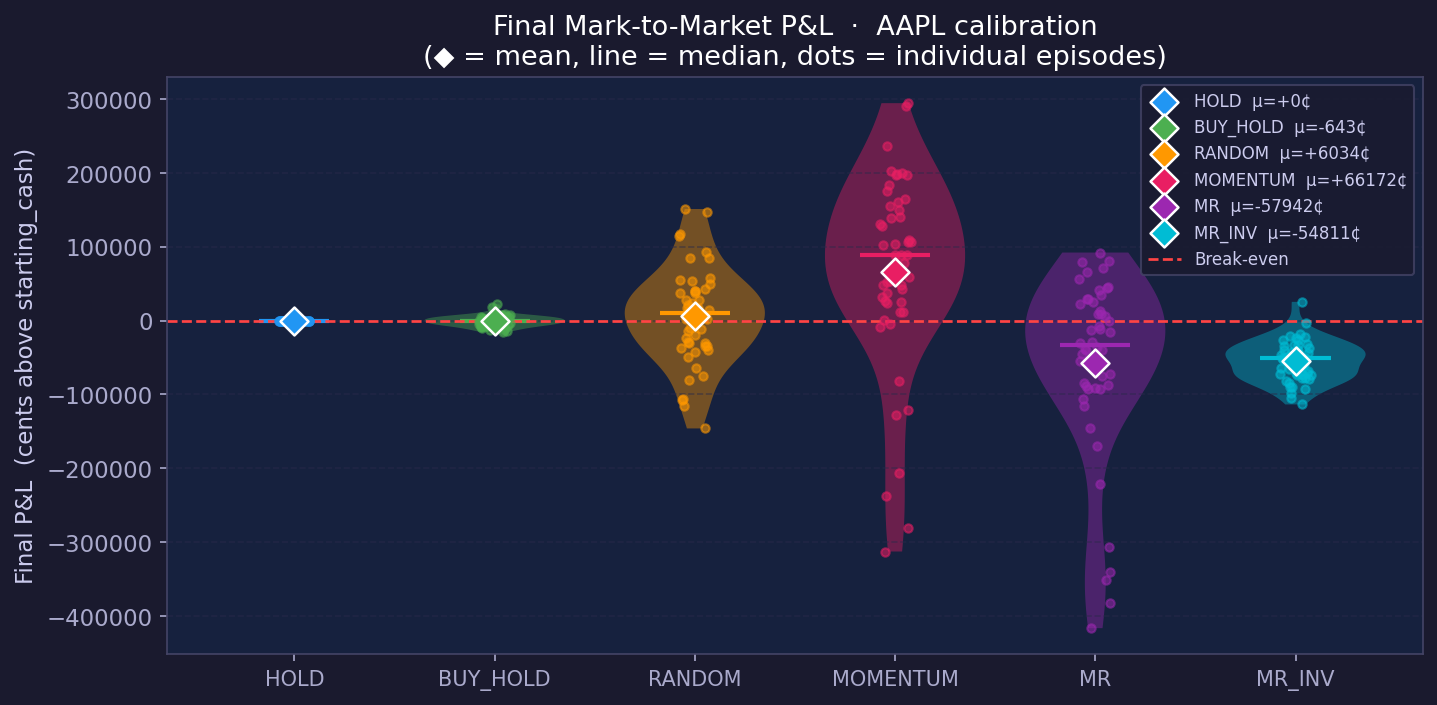
\includegraphics[width=0.95\linewidth]{../../../plots/1_m2m_pnl_distribution.png}
\caption{Final mark-to-market P\&L distribution. Diamonds denote means, median
lines show central tendency, and dots are individual episodes.}
\label{fig:baseline-pnl}
\end{figure}

\begin{figure}[H]
\centering
\begin{subfigure}{0.48\linewidth}
\centering
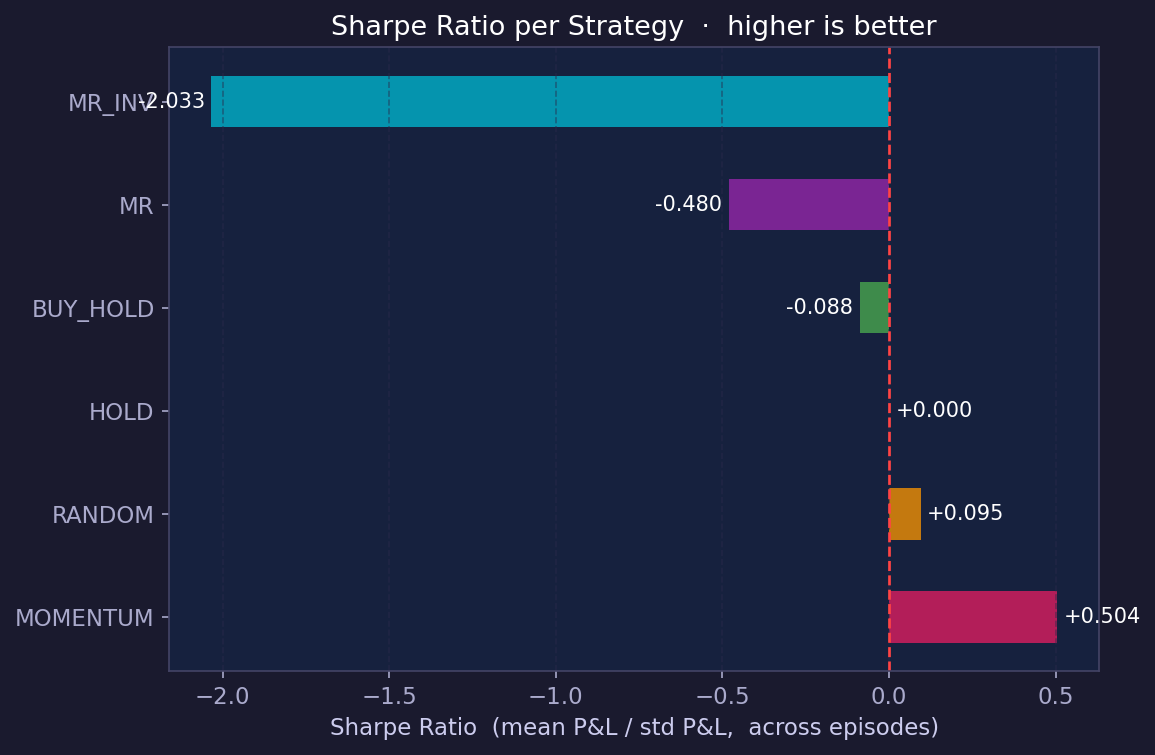
\includegraphics[width=\linewidth]{../../../plots/4_sharpe_ratio.png}
\caption{Sharpe ratio}
\end{subfigure}
\hfill
\begin{subfigure}{0.48\linewidth}
\centering
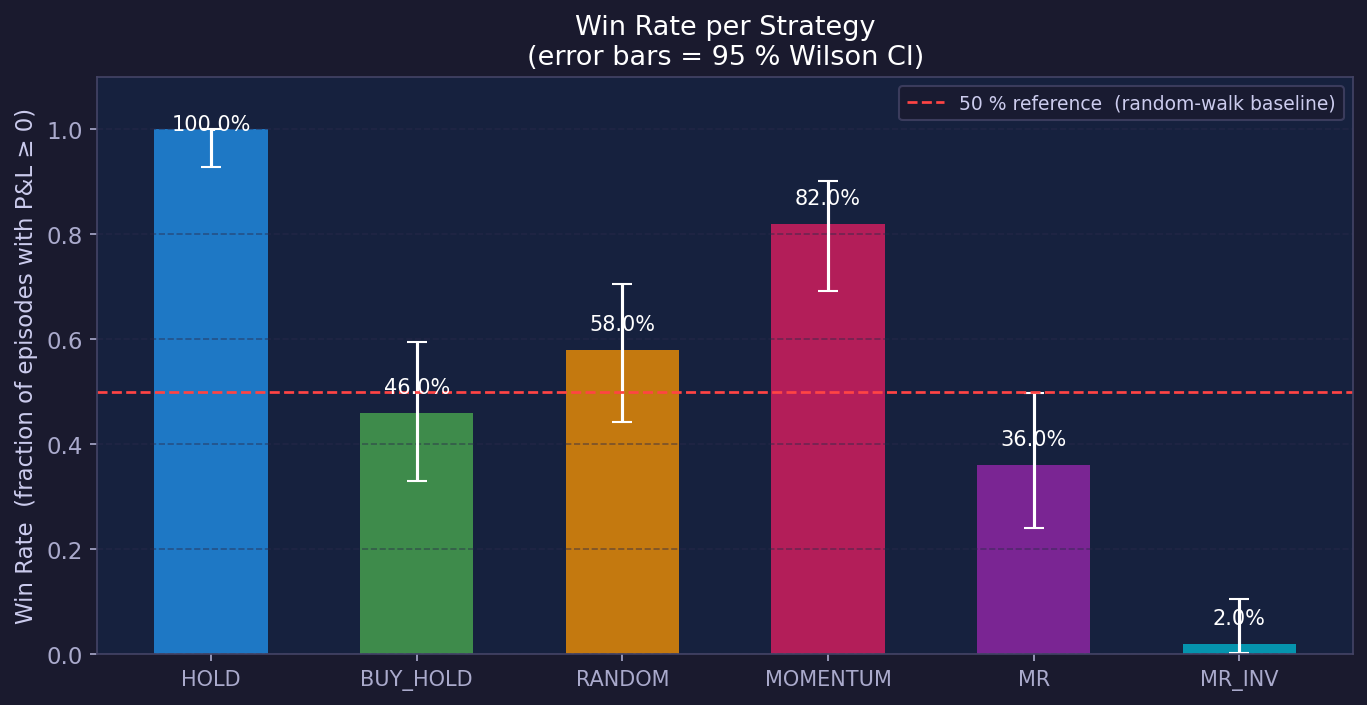
\includegraphics[width=\linewidth]{../../../plots/5_win_rate.png}
\caption{Win rate}
\end{subfigure}
\caption{Risk-adjusted and directional success metrics.}
\label{fig:baseline-sharpe-win}
\end{figure}

\begin{figure}[H]
\centering
\begin{subfigure}{0.48\linewidth}
\centering
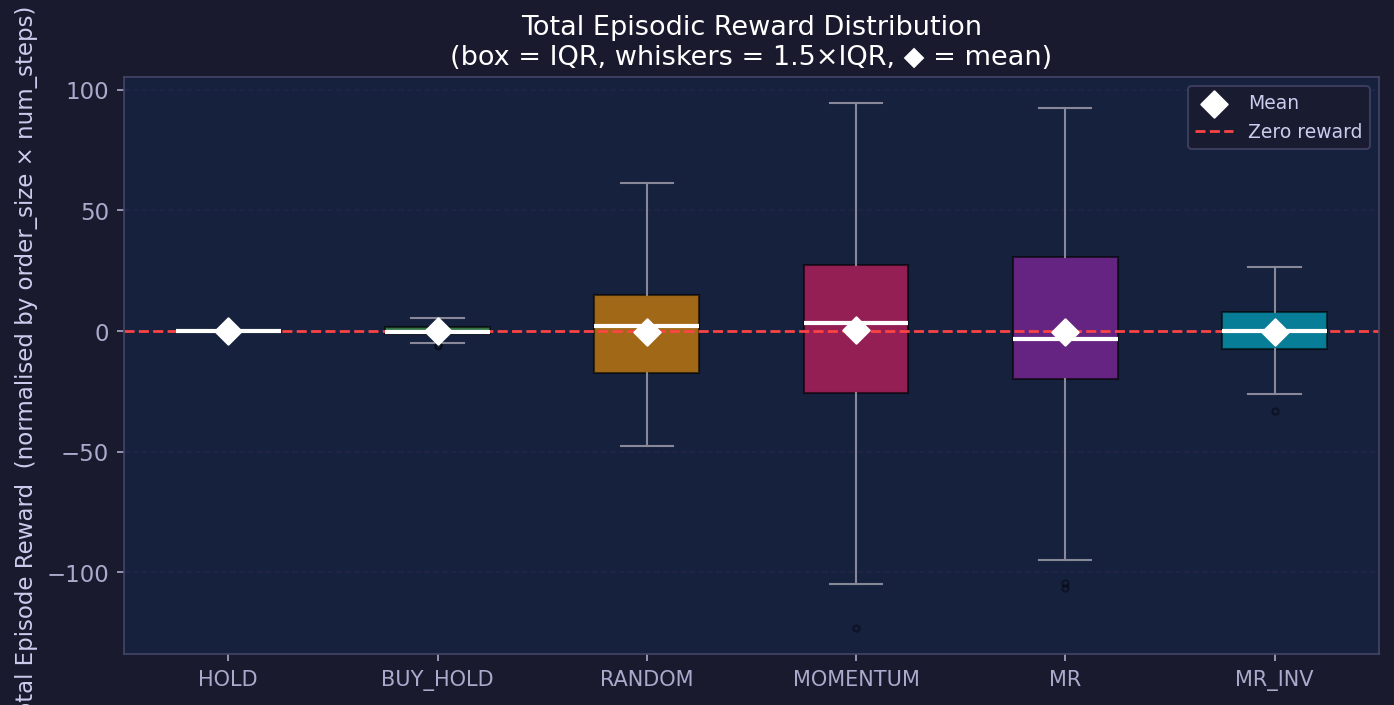
\includegraphics[width=\linewidth]{../../../plots/2_reward_distribution.png}
\caption{Episode reward}
\end{subfigure}
\hfill
\begin{subfigure}{0.48\linewidth}
\centering
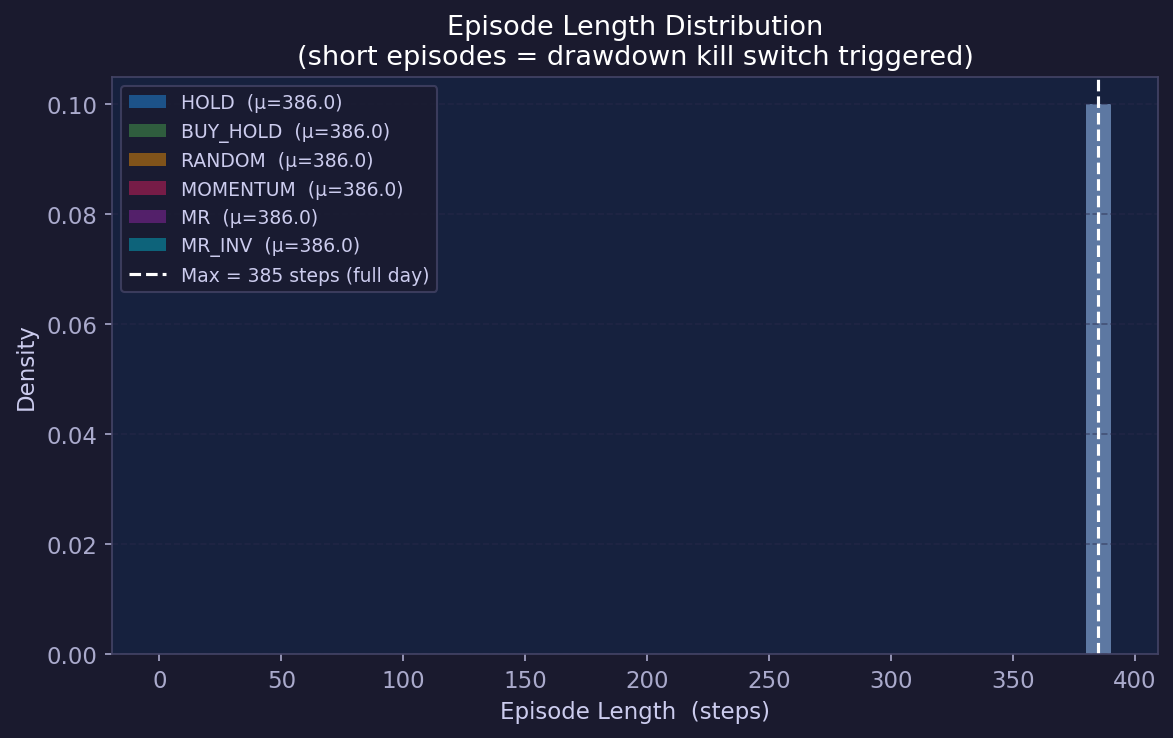
\includegraphics[width=\linewidth]{../../../plots/3_episode_length.png}
\caption{Episode length}
\end{subfigure}
\caption{Reward and termination behavior. All strategies run for the full day,
so the drawdown kill switch is not the main driver of the results.}
\label{fig:baseline-reward-length}
\end{figure}

\begin{figure}[H]
\centering
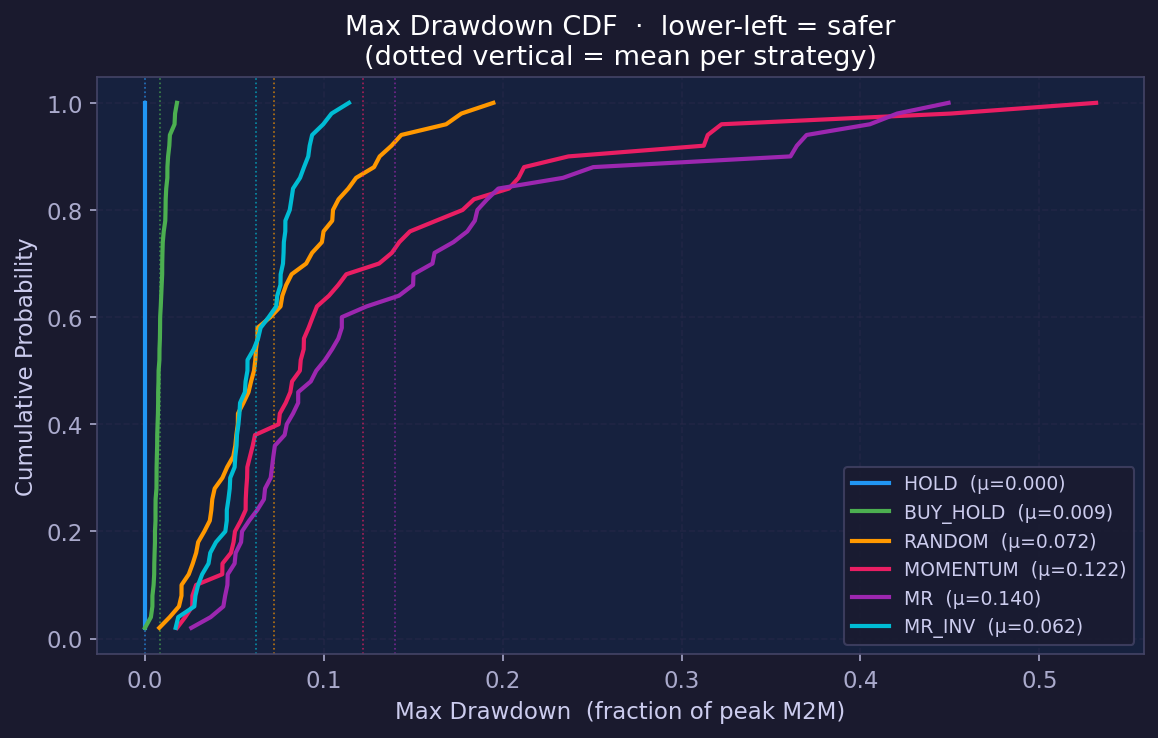
\includegraphics[width=0.78\linewidth]{../../../plots/6_max_drawdown_cdf.png}
\caption{Maximum drawdown CDF. Curves farther left are safer. \texttt{MR\_INV}
has materially lower drawdown than \texttt{MR}, but its P\&L remains negative.}
\label{fig:baseline-drawdown}
\end{figure}

\subsection{Quick Guide to the Baseline Figures}

\begin{table}[H]
\centering
\small
\begin{tabular}{p{0.22\linewidth}p{0.34\linewidth}p{0.34\linewidth}}
\toprule
Figure & What it shows & How to read it \\
\midrule
Figure~\ref{fig:baseline-pnl} &
The distribution of final P\&L for each strategy across all episodes. &
Look for strategies whose dots and mean diamond sit mostly above the red
break-even line. \texttt{MOMENTUM} is the only strategy with a clearly positive
mean and many winning episodes. \\
Figure~\ref{fig:baseline-sharpe-win} &
Two summary measures: Sharpe ratio and win rate. &
Sharpe measures risk-adjusted performance; win rate measures how often P\&L is
non-negative. This figure is the fastest ranking of the policies:
\texttt{MOMENTUM} is best, while \texttt{MR} and \texttt{MR\_INV} are poor. \\
Figure~\ref{fig:baseline-reward-length} &
Reward distribution and episode length. &
The episode-length plot confirms the strategies usually run for the full day,
so the results are not mainly caused by early termination. The reward plot
tracks the same story as P\&L because reward is based on mark-to-market changes. \\
Figure~\ref{fig:baseline-drawdown} &
The distribution of worst within-episode losses. &
Curves farther left are safer. \texttt{MR\_INV} controls drawdown better than
plain \texttt{MR}, but that risk control does not make it profitable. \\
\bottomrule
\end{tabular}
\caption{Reader's guide for the baseline figures.}
\label{tab:baseline-figure-guide}
\end{table}

\section{Parameter Sweep Results}

The sweep varies one parameter at a time and compares the same baseline
strategies. The available plots show mean final P\&L with one standard deviation
error bars. The raw \texttt{sweep\_results.json} file was not present alongside
the plots, so these conclusions should be read as qualitative interpretations of
the figures rather than exact statistical estimates.

\begin{table}[H]
\centering
\small
\begin{tabular}{p{0.24\linewidth}p{0.66\linewidth}}
\toprule
Sweep & Main interpretation \\
\midrule
\texttt{num\_value\_agents} &
The cleanest qualitative result. As value-agent count increases, \texttt{MR}
improves and \texttt{MOMENTUM} weakens, consistent with stronger fundamental
anchoring creating a more mean-reverting market. \\
\texttt{num\_momentum\_agents} &
The expected monotonic benefit to \texttt{MOMENTUM} is not clean in the plot;
variance is large and most bars overlap zero. \\
\texttt{lambda\_a} &
Higher value-agent arrival rate appears favorable to \texttt{MR}, but the
standard deviations are large. \\
\texttt{kappa}, \texttt{kappa\_oracle} &
Mean-reversion strength changes strategy rankings, but the plots are too noisy
for a strong one-parameter claim. \\
\texttt{mm\_wake\_up\_freq} &
The 60s setting looks most favorable to \texttt{MR}; 120s is worse for
\texttt{MOMENTUM}. Error bars remain wide. \\
\texttt{order\_fixed\_size}, \texttt{timestep\_duration} &
No stable monotonic transaction-cost story is visible from the current sweep. \\
\texttt{fund\_vol}, \texttt{num\_noise\_agents}, market-maker parameters &
These change opportunity and noise, but current sweep variance is large enough
that results should be treated as directional only. \\
\bottomrule
\end{tabular}
\caption{Qualitative interpretation of the one-at-a-time parameter sweep plots.}
\label{tab:sweep-interpretation}
\end{table}

\begin{figure}[H]
\centering
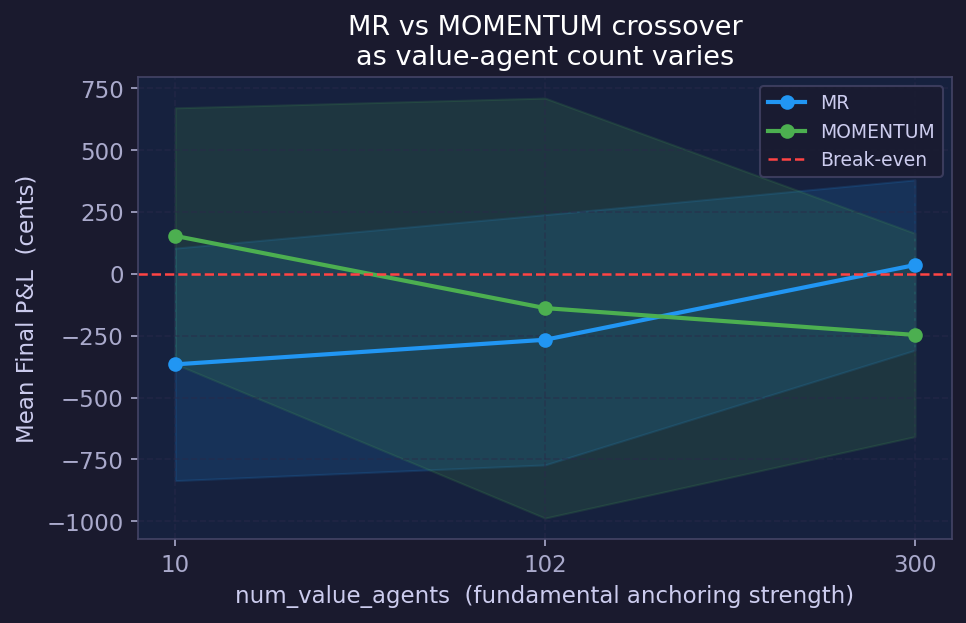
\includegraphics[width=0.75\linewidth]{../../../plots/sweep_crossover.png}
\caption{\texttt{MR} versus \texttt{MOMENTUM} as value-agent count varies.
This is the most important sweep figure: more value agents move the market
toward a mean-reverting regime.}
\label{fig:sweep-crossover}
\end{figure}

\begin{figure}[H]
\centering
\begin{subfigure}{0.48\linewidth}
\centering
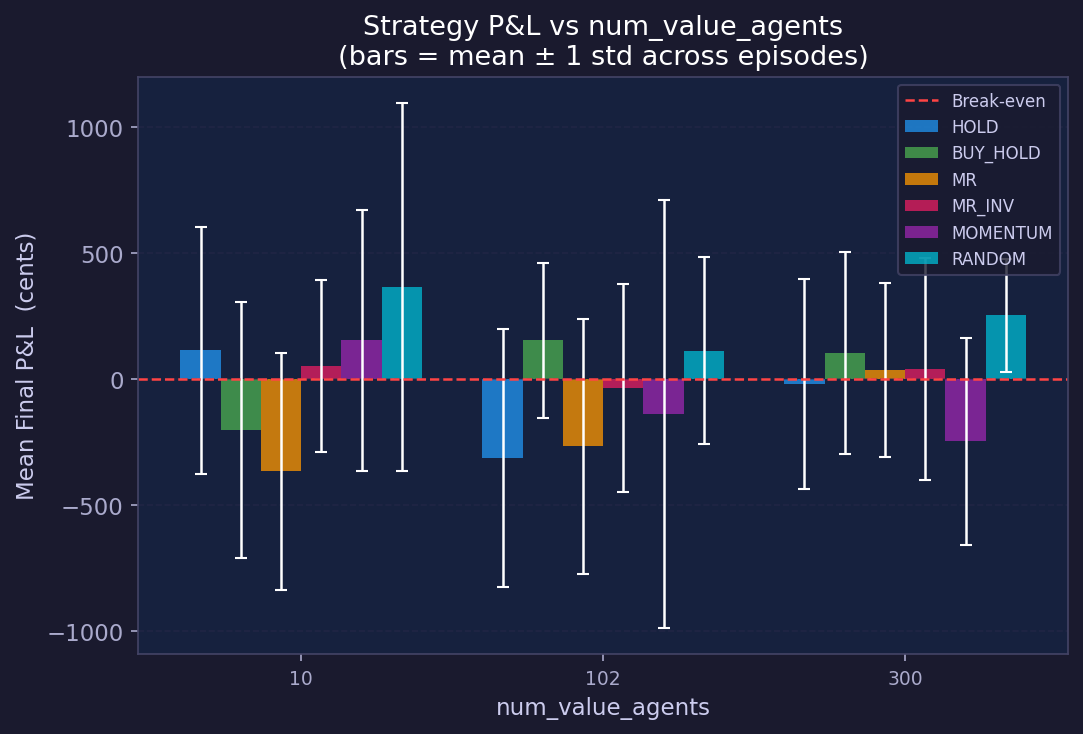
\includegraphics[width=\linewidth]{../../../plots/sweep_num_value_agents.png}
\caption{Value agents}
\end{subfigure}
\hfill
\begin{subfigure}{0.48\linewidth}
\centering
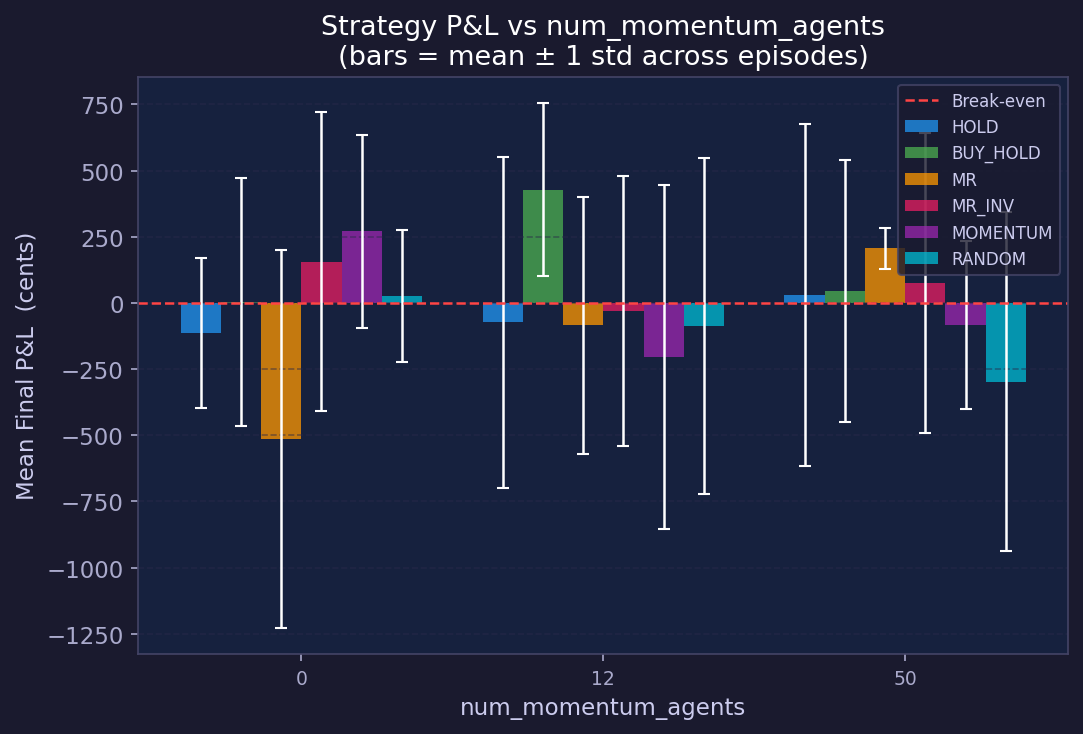
\includegraphics[width=\linewidth]{../../../plots/sweep_num_momentum_agents.png}
\caption{Momentum agents}
\end{subfigure}
\caption{Agent-population sweeps.}
\label{fig:sweep-agent-populations}
\end{figure}

\begin{figure}[H]
\centering
\begin{subfigure}{0.48\linewidth}
\centering
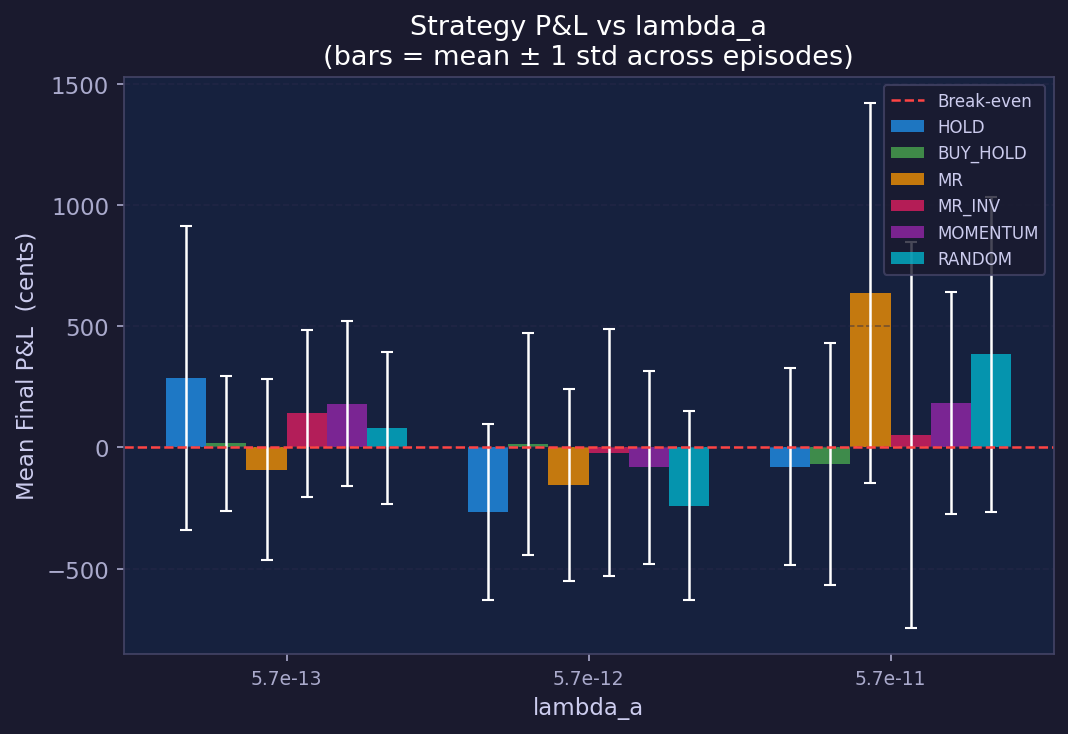
\includegraphics[width=\linewidth]{../../../plots/sweep_lambda_a.png}
\caption{\texttt{lambda\_a}}
\end{subfigure}
\hfill
\begin{subfigure}{0.48\linewidth}
\centering
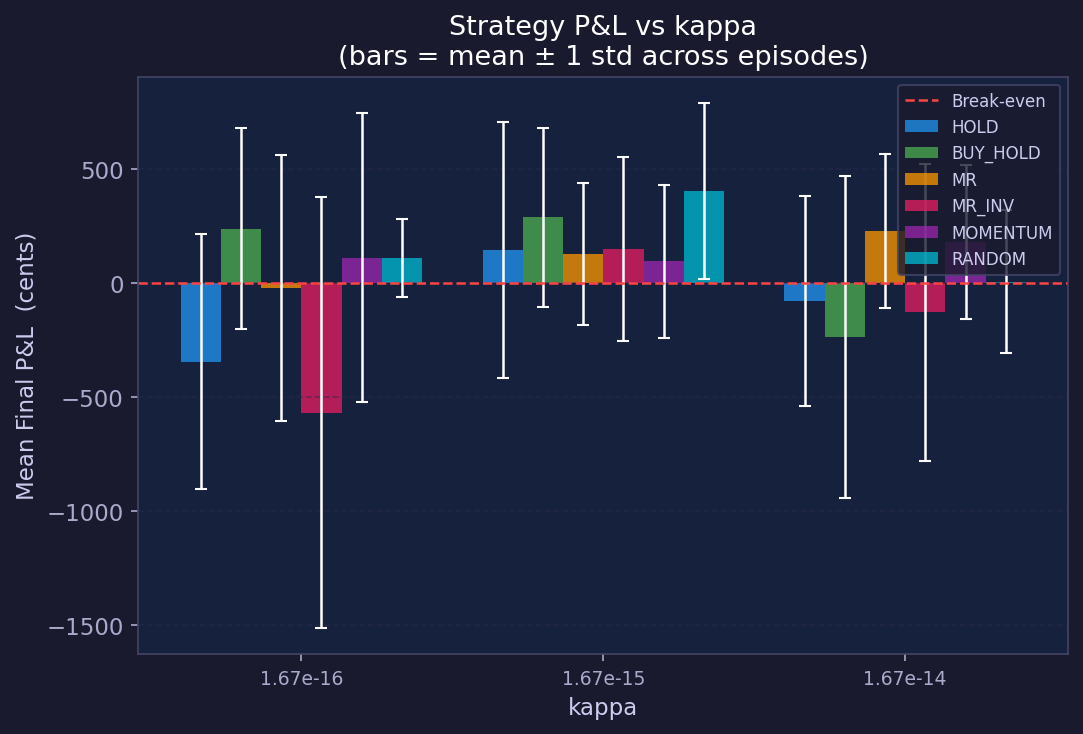
\includegraphics[width=\linewidth]{../../../plots/sweep_kappa.png}
\caption{\texttt{kappa}}
\end{subfigure}
\caption{Value-agent belief and arrival sweeps.}
\label{fig:sweep-value-beliefs}
\end{figure}

\begin{figure}[H]
\centering
\begin{subfigure}{0.48\linewidth}
\centering
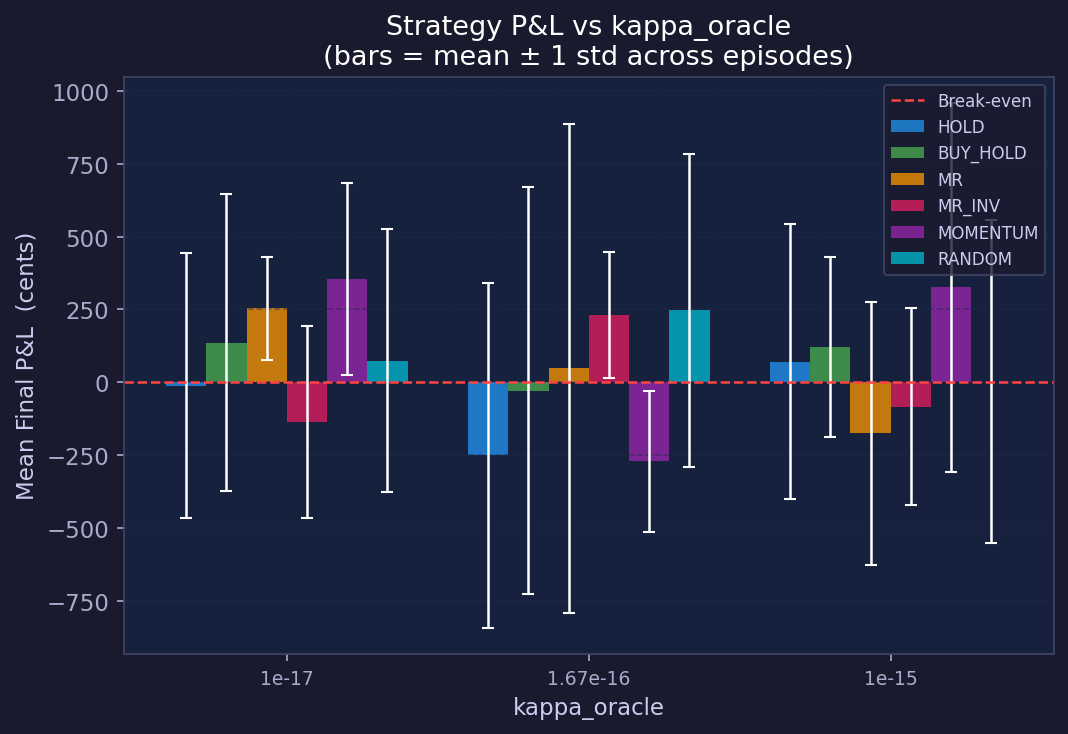
\includegraphics[width=\linewidth]{../../../plots/sweep_kappa_oracle.png}
\caption{\texttt{kappa\_oracle}}
\end{subfigure}
\hfill
\begin{subfigure}{0.48\linewidth}
\centering
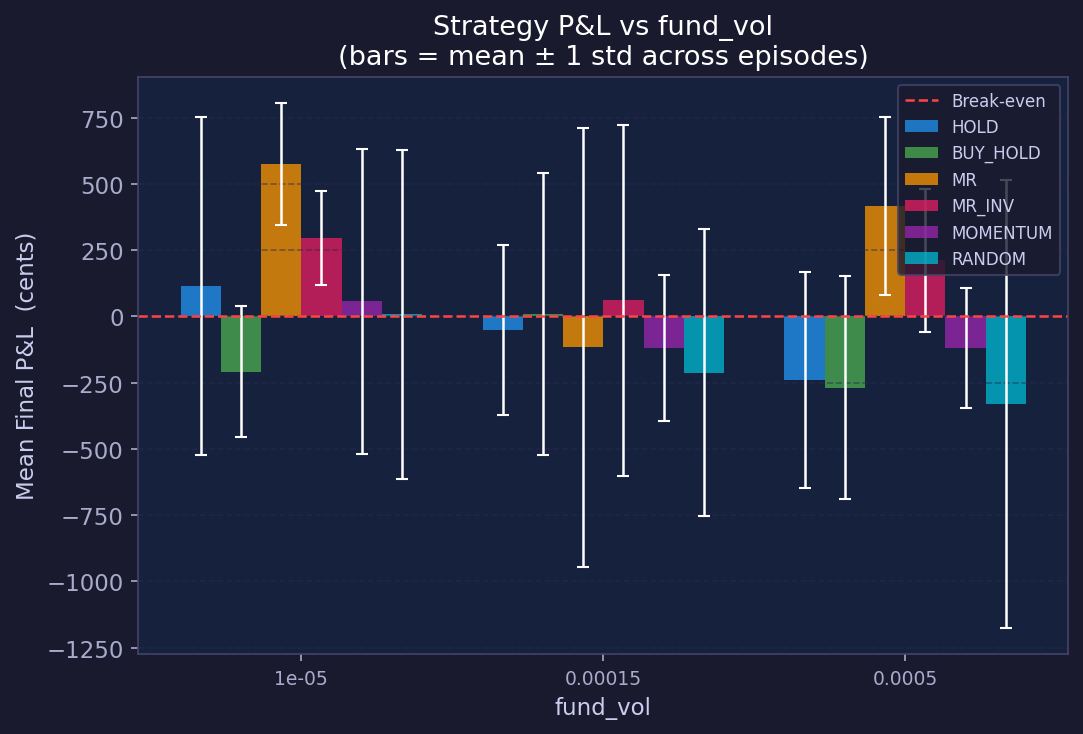
\includegraphics[width=\linewidth]{../../../plots/sweep_fund_vol.png}
\caption{\texttt{fund\_vol}}
\end{subfigure}
\caption{Oracle fundamental-process sweeps.}
\label{fig:sweep-oracle}
\end{figure}

\begin{figure}[H]
\centering
\begin{subfigure}{0.48\linewidth}
\centering
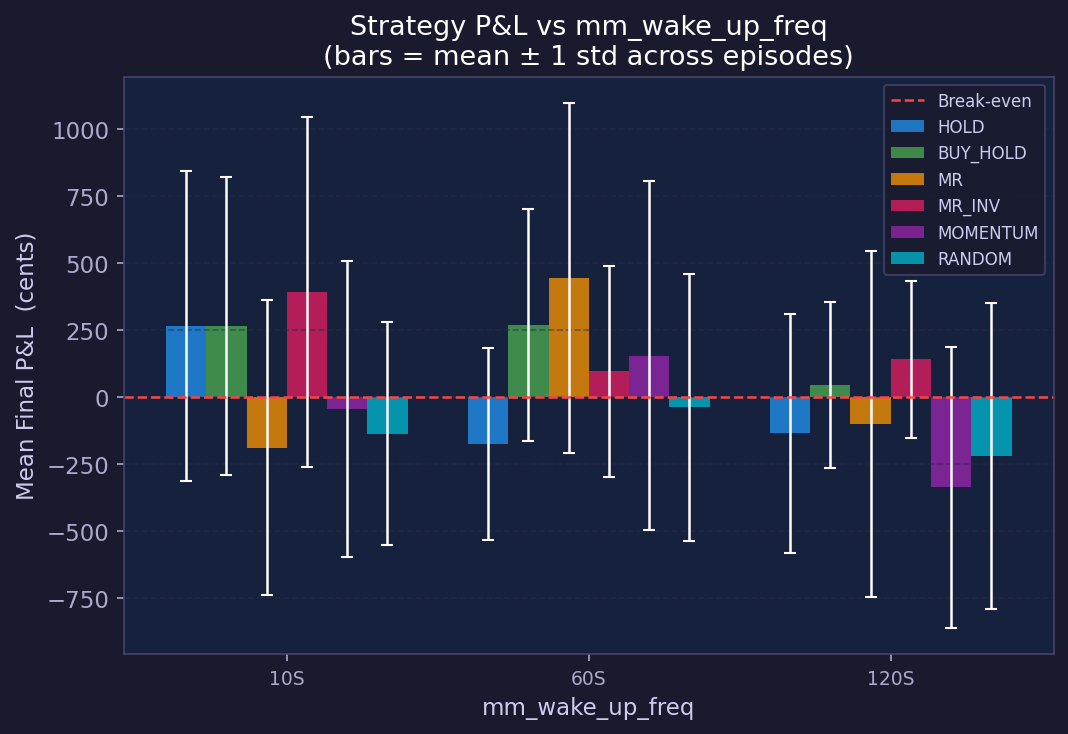
\includegraphics[width=\linewidth]{../../../plots/sweep_mm_wake_up_freq.png}
\caption{Wake-up frequency}
\end{subfigure}
\hfill
\begin{subfigure}{0.48\linewidth}
\centering
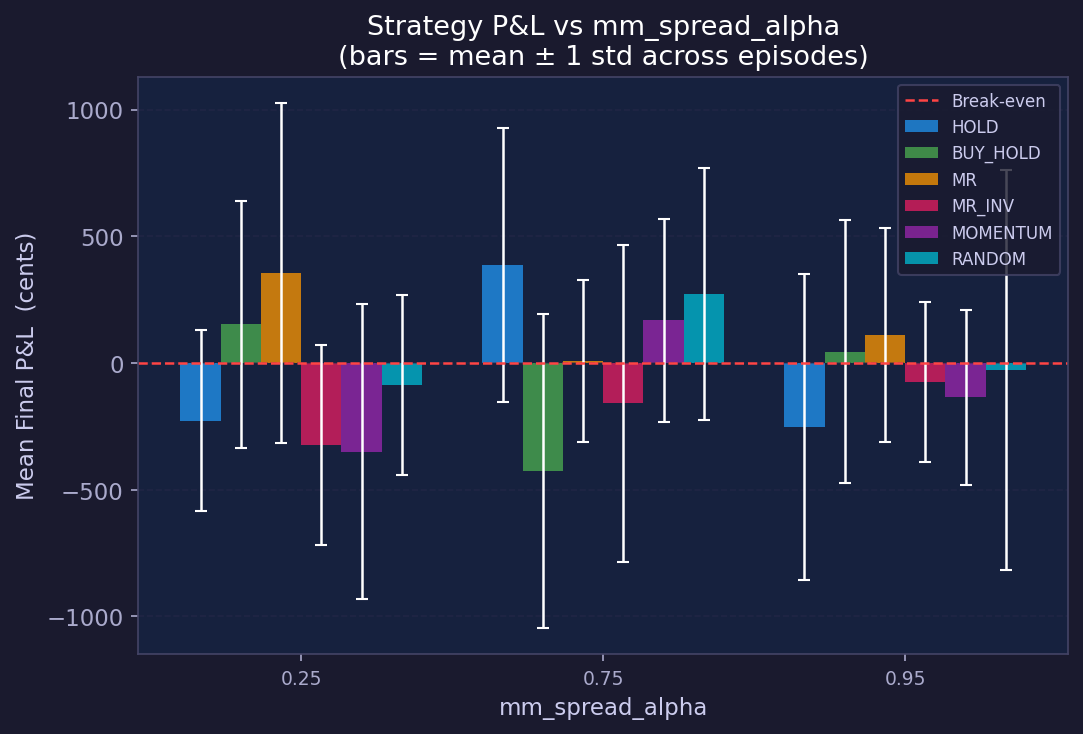
\includegraphics[width=\linewidth]{../../../plots/sweep_mm_spread_alpha.png}
\caption{Spread alpha}
\end{subfigure}
\caption{Market-maker timing and spread-adaptation sweeps.}
\label{fig:sweep-mm-timing}
\end{figure}

\begin{figure}[H]
\centering
\begin{subfigure}{0.48\linewidth}
\centering
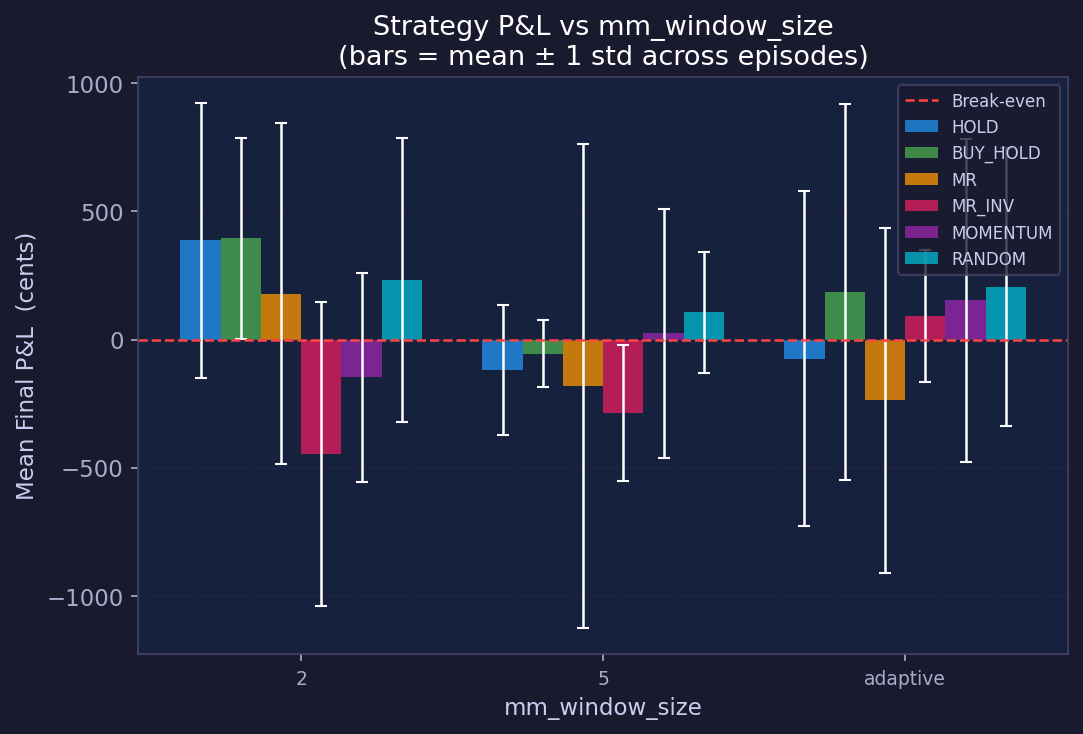
\includegraphics[width=\linewidth]{../../../plots/sweep_mm_window_size.png}
\caption{Window size}
\end{subfigure}
\hfill
\begin{subfigure}{0.48\linewidth}
\centering
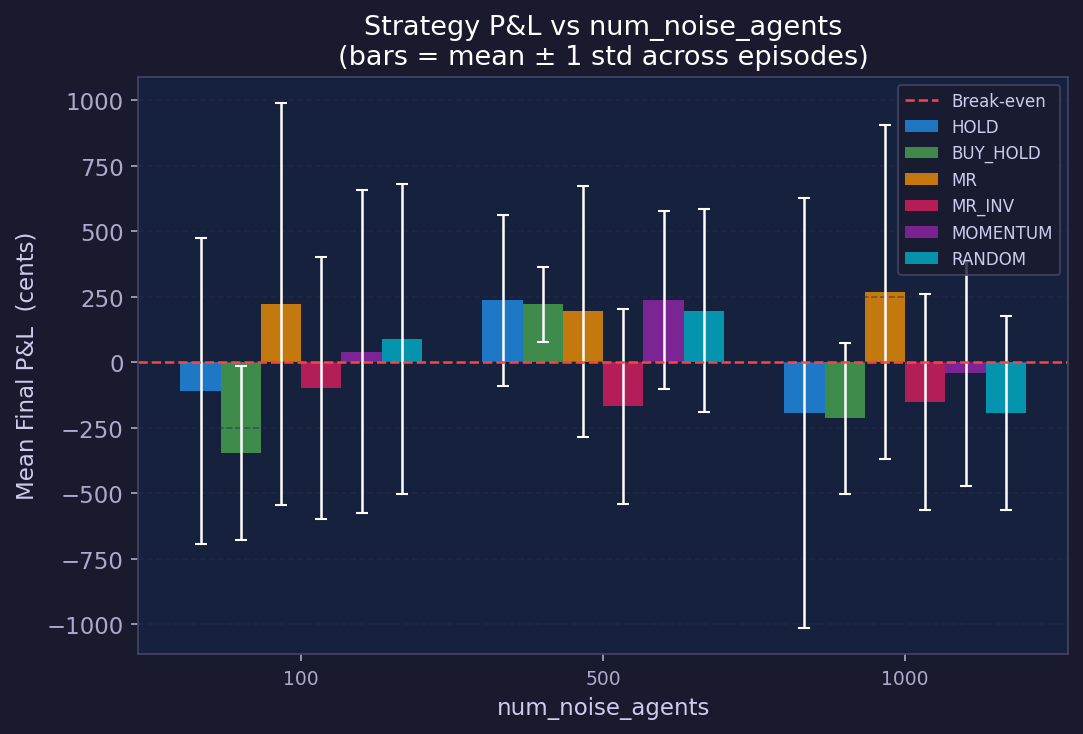
\includegraphics[width=\linewidth]{../../../plots/sweep_num_noise_agents.png}
\caption{Noise agents}
\end{subfigure}
\caption{Liquidity and noise sweeps.}
\label{fig:sweep-liquidity-noise}
\end{figure}

\begin{figure}[H]
\centering
\begin{subfigure}{0.48\linewidth}
\centering
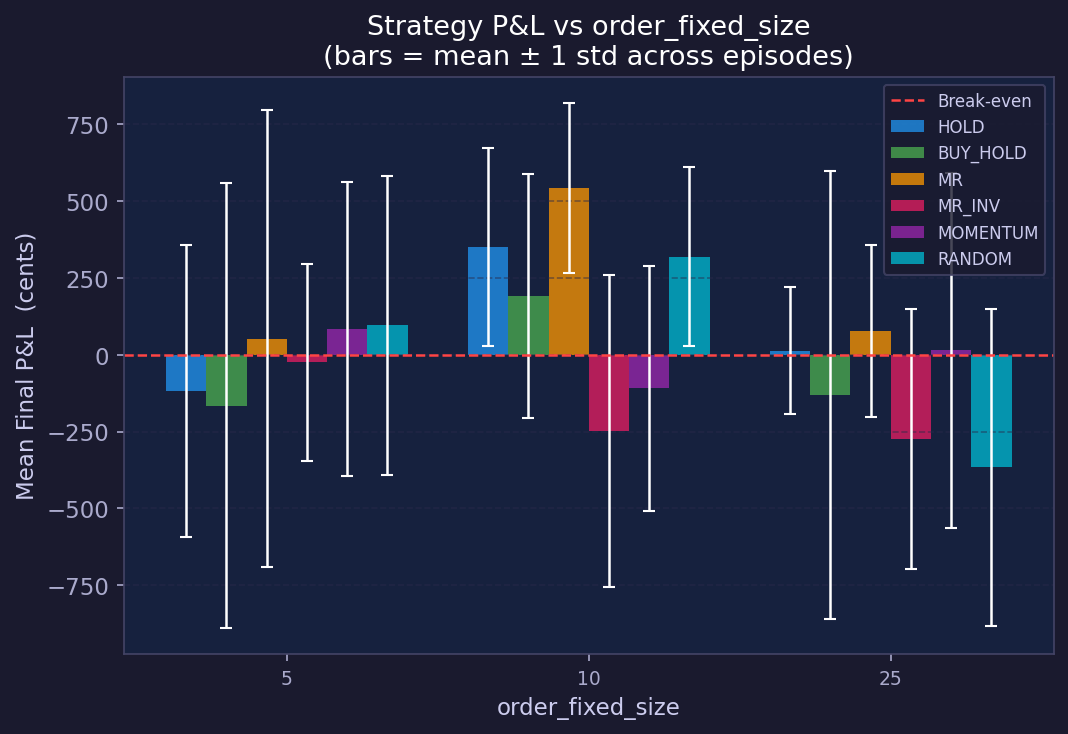
\includegraphics[width=\linewidth]{../../../plots/sweep_order_fixed_size.png}
\caption{Order size}
\end{subfigure}
\hfill
\begin{subfigure}{0.48\linewidth}
\centering
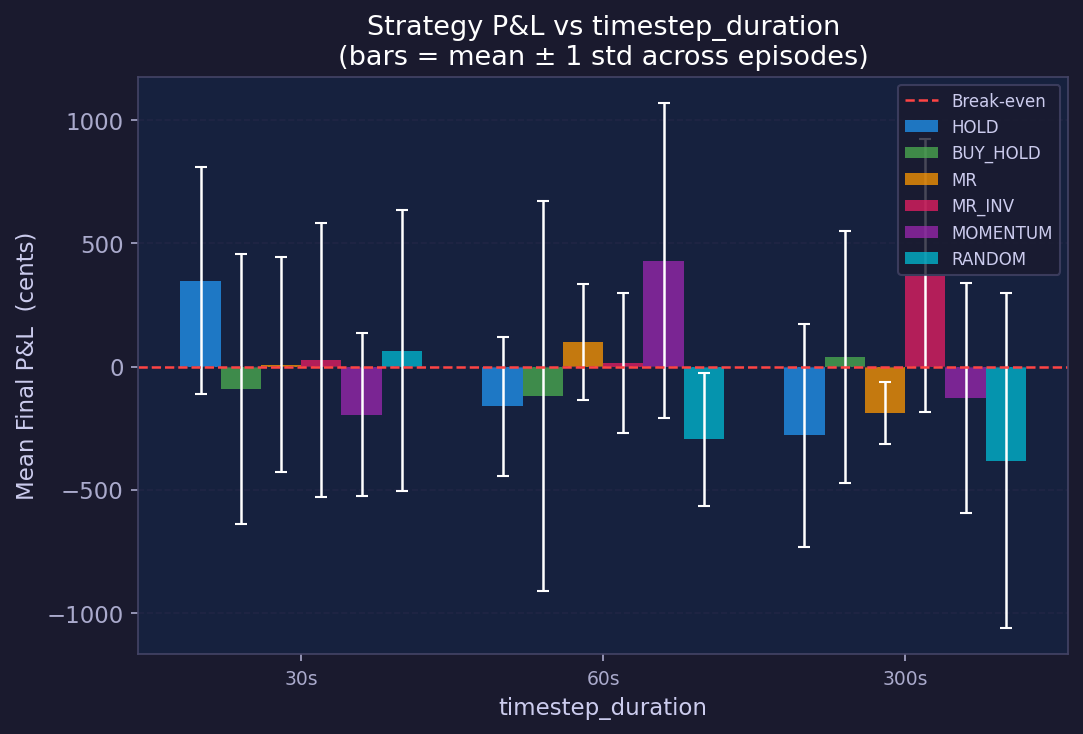
\includegraphics[width=\linewidth]{../../../plots/sweep_timestep_duration.png}
\caption{Timestep duration}
\end{subfigure}
\caption{Environment-level action-frequency and order-size sweeps.}
\label{fig:sweep-env}
\end{figure}

\subsection{Quick Guide to the Sweep Figures}

\begin{table}[H]
\centering
\small
\begin{tabular}{p{0.22\linewidth}p{0.34\linewidth}p{0.34\linewidth}}
\toprule
Figure & What it varies & What to take away \\
\midrule
Figure~\ref{fig:sweep-crossover} &
Only the number of value agents, comparing \texttt{MR} against
\texttt{MOMENTUM}. &
This is the most important sweep figure. More value agents make the market more
fundamentally anchored, which improves \texttt{MR} and weakens
\texttt{MOMENTUM}. \\
Figure~\ref{fig:sweep-agent-populations} &
The number of value agents and momentum agents. &
These plots ask whether changing the hidden trader population changes which
strategy works. The value-agent trend is the cleanest evidence that regime
composition matters. \\
Figure~\ref{fig:sweep-value-beliefs} &
Value-agent arrival rate \texttt{lambda\_a} and value-agent belief strength
\texttt{kappa}. &
These parameters control how aggressively value agents react to deviations from
fundamental value. The plots are noisy, but they help identify candidate
mean-reverting regimes for future RL training. \\
Figure~\ref{fig:sweep-oracle} &
The true fundamental process: \texttt{kappa\_oracle} and \texttt{fund\_vol}. &
These change how the underlying fundamental value moves. Larger changes can
create more opportunity, but also more risk; wide error bars mean the current
sweep is not decisive. \\
Figure~\ref{fig:sweep-mm-timing} &
Market-maker wake-up frequency and spread adaptation. &
These parameters control liquidity refresh and spread behavior. They matter
because every active policy crosses the spread when it buys or sells. \\
Figure~\ref{fig:sweep-liquidity-noise} &
Market-maker window size and the number of noise agents. &
These plots probe liquidity and noisy order flow. They mostly show high
variance, so they should be treated as diagnostic rather than conclusive. \\
Figure~\ref{fig:sweep-env} &
Order size and timestep duration. &
These are environment-level controls. They change how often the agent trades
and how large each trade is, so they affect transaction costs and signal
granularity. \\
\bottomrule
\end{tabular}
\caption{Reader's guide for the parameter sweep figures.}
\label{tab:sweep-figure-guide}
\end{table}

\section{Takeaways}

The results should be read as a chain of evidence:

\begin{enumerate}
    \item \textbf{First, the default market has a clear winner.}
    In the baseline table, \texttt{MOMENTUM} has the highest mean P\&L, the
    best Sharpe ratio, and the highest non-trivial win rate. The
    mean-reversion strategies, \texttt{MR} and \texttt{MR\_INV}, lose money on
    average. This tells us that the default AAPL-calibrated market rewards
    short-horizon momentum more than mean reversion.

    \item \textbf{Second, this is not just because all active trading works.}
    \texttt{RANDOM} trades actively but performs much worse than
    \texttt{MOMENTUM}. That means the momentum strategy is using a useful
    signal, not merely benefiting from taking more trades.

    \item \textbf{Third, changing the market composition changes the story.}
    In the value-agent sweep, increasing \texttt{num\_value\_agents} makes
    \texttt{MR} improve and makes \texttt{MOMENTUM} weaken. This is important:
    it suggests that different hidden market regimes favor different trading
    behavior.

    \item \textbf{That is exactly why belief estimation is useful.}
    If the best action depends on whether the market is momentum-heavy or
    value-agent-heavy, then an RL trader should not use one fixed policy for
    every regime. It should estimate the current regime from public market
    history and condition its policy on that belief.

    \item \textbf{The immediate next step is to build those regimes explicitly.}
    We should train and evaluate two agents across several known ABIDES market
    compositions: a standard RL trader that sees only market observations, and
    a belief-aware trader that also receives an estimated regime vector. The
    belief-aware trader should be judged by both trading performance and how
    well its inferred beliefs match the known simulated market composition.
\end{enumerate}

The main caveat is that the sweep plots are still noisy. They are strong enough
to motivate the next experiment, especially the value-agent result, but most
individual parameter effects need more episodes or the raw sweep table before
they should be treated as final statistical claims.

This also translates to the main multi-agent experiment. The trading agent is
not trying to identify one named opponent. Instead, it observes the public
footprint of many hidden agents acting together: prices, spreads, imbalance,
and returns. The belief module should therefore estimate the current
multi-agent market composition, such as ``mostly momentum,'' ``mostly value,''
or ``mixed.'' If different compositions favor different trading behavior, as
the sweep suggests, then conditioning the RL policy on that belief is the right
multi-agent analogue of estimating a partner type in a cooperative game.

\end{document}
